% !TEX TS-program = xelatex
% !TEX encoding = UTF-8 Unicode

% Lecture Template for ME3001-001-Tristan Hill - Spring 2017 - Fall 2017 - Fall 2020
% Mechanical Engineering Analysis with MATLAB
% Module 4 - Eigenvalues and Eigenvectors
% Topic 1 - What is an Eigen Value?

\documentclass[fleqn]{beamer} % for presentation (has nav buttons at bottom)

\usepackage{/home/thill/Documents/lectures/analysis_lectures/analysis_lectures}

\newcommand{\MNUM}{3\hspace{2mm}} % Module number
\newcommand{\TNUM}{1\hspace{2mm}} % Topic number 
\newcommand{\moduletitle}{Eigenvalues and Eigenvectors} % Titles and Stuff
\newcommand{\topictitle}{What is an Eigenvalue and Eigenvector?} 

\newcommand{\sectiontitleI}{Mathematical Definition of Eigenvalue and Eigenvector} % More Titles and Stuff
\newcommand{\sectiontitleII}{Standard form Eigenvalue Problem}
\newcommand{\sectiontitleIII}{The Geometrical Explanation}
\newcommand{\sectiontitleIV}{A Simple Example by Hand}


\author{ME3001 - Mechanical Engineering Analysis}
\title{Module \MNUM - \moduletitle}
\date{Mechanical Engineering\vspc Tennessee Technological University}

\begin{document}

\lstset{language=MATLAB,basicstyle=\ttfamily\small,showstringspaces=false}

\frame{\titlepage \center\begin{framed}\Large \textbf{Topic \TNUM - \topictitle}\end{framed} \vspace{5mm}}

% Section 0 - Outline
\frame{
	
	\large \textbf{Topic \TNUM - \topictitle} \vspace{3mm}\\
	
	\begin{itemize}
	
		\item \sectiontitleI    \vspc % Section I
		\item \sectiontitleII 	\vspc % Section II
		\item \sectiontitleIII 	\vspc %Section III
		\item \sectiontitleIV 	\vspc %Section IV
	
	\end{itemize}

}


\section{\sectiontitleI}

\frame{ \small
  \frametitle{\sectiontitleI}
  	
\textbf{Did you study this in calculus? Differential Equations?} \vspace{3mm}

			In linear algebra, an eigenvector or characteristic vector of a linear transformation is a non-zero vector whose direction does not change when that linear transformation is applied to it. More formally, if $T$ is a linear transformation from a vector space $V$ over a field $F$ into itself and $v$ is a vector in $V$ that is not the zero vector, then $v$ is an eigenvector of $T$ if $T(v)$ is a scalar multiple of $v$. This condition can be written as the equation\\

\scalebox{1.5}{$T({\bf v})=\lambda{\bf v}$}\\

}


\frame{ \small
  \frametitle{\sectiontitleI}
  	
where $\lambda$ is a scalar in the field $F$, known as the eigenvalue, characteristic value, or characteristic root associated with the eigenvector $v$.

If the vector space $V$ is finite-dimensional, then the linear transformation $T$ can be represented as a square matrix $A$, and the vector $v$ by a column vector, rendering the above mapping as a matrix multiplication on the left hand side and a scaling of the column vector on the right hand side in the equation.\\

\scalebox{1.5}{$[A]{\bf v}=\lambda{\bf v}$}\\

}



\section{\sectiontitleII}

\frame{ \small
  \frametitle{\sectiontitleII}
  
  \scalebox{1.0}{\parbox{.5\linewidth}{
			\[ \left( \begin{array}{cccc}
			a_{11}  & a_{12} & ...& a_{1n} \\
			a_{21} & a_{22}  & ...& a_{2n} \\
			&.&&\\
			&.&&\\
			a_{n1} & a_{n2} & ...& a_{nn} \end{array} \right) \times \left[ \begin{array}{c}
			x_1 \\
			x_2 \\
			.\\
			.\\
			x_n \end{array} \right] = \lambda\left[ \begin{array}{c}
			x_1 \\
			x_2 \\
			.\\
			.\\
			x_n \end{array} \right]\] 
			}}
  	 	\scalebox{1.0}{\parbox{.5\linewidth}{
			\[ \left(\left[ \begin{array}{cccc}
			a_{11}  & a_{12} & ...& a_{1n} \\
			a_{21} & a_{22}  & ...& a_{2n} \\
			&.&&\\
			&.&&\\
			a_{n1} & a_{n2} & ...& a_{nn} \end{array} \right]-\lambda\left[ \begin{array}{cccc}
			1  & 0 & ...& 0 \\
			0 & 1  & ...& 0 \\
			0 & 0  & 1 & 0 \\
			&.&&\\
			0 & 0 & ...& 1 \end{array} \right]\right) \times \left[ \begin{array}{c}
			x_1 \\
			x_2 \\
			.\\
			.\\
			x_n \end{array} \right] = \left[ \begin{array}{c}
			0\\
			0 \\
			.\\
			.\\
			0 \end{array} \right]\] 
			}}

		 	
  
  }

\frame{ \small
  \frametitle{\sectiontitleII}
		The Equations \\\\
		  \scalebox{1.0}{$(a_{11}-\lambda) x_1 + a_{12} x_{2} + ... + a_{1n} x_n = 0 $} \vspace{2mm}
		  \scalebox{1.0}{$a_{21} x_1 + (a_{22}-\lambda)  x_{2} + ... + a_{2n} x_n = 0 $} \\
		  \scalebox{1.0}{$\hspace{20mm}.$}\\
		  \scalebox{1.0}{$\hspace{20mm}.$}\\
		  \scalebox{1.0}{$a_{n1} x_1 + a_{n2} x_{2} + ... + (a_{nn}-\lambda) x_n = 0 $} \\	
		  
		 The Matrix Form 	\\
		 	\scalebox{1.0}{\parbox{.5\linewidth}{
			\[ \left( \begin{array}{cccc}
			(a_{11}-\lambda)  & a_{12} & ...& a_{1n} \\
			a_{21} & (a_{22}-\lambda)  & ...& a_{2n} \\
			&.&&\\
			&.&&\\
			a_{n1} & a_{n2} & ...& (a_{nn}-\lambda) \end{array} \right) \times \left[ \begin{array}{c}
			x_1 \\
			x_2 \\
			.\\
			.\\
			x_n \end{array} \right] = \left[ \begin{array}{c}
			0\\
			0 \\
			.\\
			.\\
			0 \end{array} \right]\] 
			}}		
}




\section{\sectiontitleIII}

\frame{ \small
  \frametitle{\sectiontitleIII}
 \textbf{Let us look at the second matrix form more closely}\\

\scalebox{1.0}{$([A]-\lambda[I])\{x\}=\{0\}$} \\

First we need to realize that this matrix system is {\it Homogeneous}. This follows a different rule regarding the existence of a solution.\\
 A {\it Homogeneous} system has a non-trivial solution if and only if the determinant of the coefficient matrix is zero.\\

\scalebox{1.0}{$|[A]|=0$}\\

Therefore\\
\scalebox{1.0}{$|[A]-\lambda[I]|=0$} \\

This leads to a long $n^{th}$ order polynomial in terms of $\lambda$. This will have $n$ roots which may be real or complex.


  }
  \frame{ \small
  \frametitle{\sectiontitleIII}
3x3 example \\
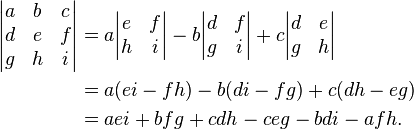
\includegraphics[scale=.5]{lecture5_fig1.png}
	
	
  }
  
  \section{\sectiontitleIV}

  \frame{ \small
  \frametitle{\sectiontitleIV}
  Example with 2D Vectors \vspace{50mm}
	
  }
  \frame{ \small
  \frametitle{\sectiontitleIII}
  Example with 2D Vectors \vspace{50mm}
	
  }
   \frame{ \small
  \frametitle{\sectiontitleIII}
  Example with 2D Vectors \vspace{50mm}
	
  }
\end{document}

%
%\begin{itemize}
%
%	\item  \textbf{\LARGE What is a Linear Equation}
%		\LARGE
%		\begin{itemize}
%			\item ``A linear equation is an algebraic equation in which each term is either a constant or the product of a constant and a single variable'' - Wikipedia \\ \vspace{10mm}
%			
%			\item slope intercept form	\\\vspace{20mm}
%			
%			\item does not contain \\\vspace{20mm}
%		\end{itemize}	
%
%	\item \textbf{\LARGE What is a System of Linear Equations?}
%		\begin{itemize}
%			\item multiple linear equations with... \\\vspace{20mm}
%			\item also known as... \\\vspace{20mm}				
%		\end{itemize}
%
%\newpage
%\item \textbf{\LARGE General Form of  A Linear System}
%	\begin{itemize}
%		\item The System of Linear Equations \\ \\
%		  \scalebox{1.5}{$a_{11} x_1 + a_{12} x_{2} + ... + a_{1n} x_n = b_1 $} \\
%		  \scalebox{1.5}{$a_{21} x_1 + a_{22} x_{2} + ... + a_{2n} x_n = b_2 $} \\
%		  \scalebox{1.5}{$\hspace{20mm}.$}\\
%		  \scalebox{1.5}{$\hspace{20mm}.$}\\
%		  \scalebox{1.5}{$\hspace{20mm}.$}\\		
%		  \scalebox{1.5}{$a_{n1} x_1 + a_{n2} x_{2} + ... + a_{nn} x_n = b_n $} \\\vspace{20mm}		
%		  
%		 
%		 \item The Matrix Form of the System 	\\\\
%		 	\scalebox{1.5}{\parbox{.5\linewidth}{
%			\[ \left( \begin{array}{cccc}
%			a_{11} & a_{12} & ...& a_{1n} \\
%			a_{21} & a_{22} & ...& a_{2n} \\
%			&.&&\\
%			&.&&\\
%			a_{n1} & a_{n2} & ...& a_{nn}\end{array} \right) \times \left[ \begin{array}{c}
%			x_1 \\
%			x_2 \\
%			.\\
%			.\\
%			x_n \end{array} \right] = \left[ \begin{array}{c}
%			b_1 \\
%			b_2 \\
%			.\\
%			.\\
%			b_n \end{array} \right]\] 
%			}} \vspace{10mm}\\
%			
%			 \item The Solution to the System of Equations	\\
%%		\newpage 
%%		 \item Matrix Multiplication  \\ \vspace{5mm}
%%		 
%%		 	 \scalebox{1.5}{ $C = A \times B \hspace{20mm} c_{ij}=\Sigma_{k=1}^n a_{ik}\times b_{kj}$} \\ \vspace{50mm}
%%		 
%%		 
%%		 \item Conformability \\ \vspace{30mm}
%%		 
%%		 
%%		 
%%	\end{itemize}
%%
%%\newpage
%%\item \textbf{\LARGE Basic Example}
%%
%%
%%\newpage
%%\item \textbf{\LARGE Basic Linear Algebra in MATLAB}
%%
%%	\begin{itemize}
%%
%%		\item \textbf{ \LARGE Useful Functions}\vspace{10mm}\\
%%
%%		\begin{multicols}{2}
%%			\scalebox{1.5}{{\fontfamily{qcr}\selectfont  \hspace{5mm} det()}} \VC \\
%%			\scalebox{1.5}{{\fontfamily{qcr}\selectfont  \hspace{5mm} rank()}} \VC\\
%%			\scalebox{1.5}{{\fontfamily{qcr}\selectfont  \hspace{5mm} inv()}} \VC\\
%%			\scalebox{1.5}{{\fontfamily{qcr}\selectfont  \hspace{5mm} `}} \VC\\
%%			
%%			\scalebox{1.5}{Determinant}\VC\\
%%			\scalebox{1.5}{Rank}\VC\\	
%%			\scalebox{1.5}{Inverse}\VC\\
%%			\scalebox{1.5}{Transpose}\VC\\
%%		
%%		\end{multicols}
%%
%
%\end{itemize}
%
%
%\newpage
%
%\item \textbf{\LARGE A Mechanical Engineering Example - Geometry}\\\\	
%		
%		As a group we are going to setup 2 small examples. \\\\
%		\begin{description}
%		\item [Example 1:] Intersection of 2 Lines.  \hspace{5mm} \scalebox{1.25}{ax+by=c} \\
%		\begin{enumerate}
%		
%			\item Write the individual equations. \vspace{100mm}
%		
%			\item Organize the equations.
%
%\newpage 
%		
%			\item Cast the system into matrix form. \vspace{140mm}
%			
%			\item Solve the system. \\
%			\begin{itemize}
%				\item \hspace{10mm} \\
%				\item \hspace{10mm} \\
%				\item \hspace{10mm} \\
%			\end{itemize}
%		
%		\end{enumerate}
%		
%		\newpage 
%		\item [Example 2:] Intersection of 3 Planes.  \scalebox{1.25}{ax+by+cz=d} \\\\
%		\begin{enumerate}
%		
%			\item Write the individual equations. \vspace{100mm}
%		
%			\item Organize the equations.
%
%\newpage 
%		
%			\item Cast the system into matrix form. \vspace{140mm}
%			
%			\item Solve the system. \\
%			\begin{itemize}
%				\item \hspace{10mm} \\
%				\item \hspace{10mm} \\
%				\item \hspace{10mm} \\
%			\end{itemize}
%		
%		\end{enumerate}
%		
%		
%
%		\end{description}
%
%		
%
%
%
%
%\newpage 
%
%	%\item \textbf{ \LARGE REMINDER - Homework 1 was due Friday, Turn it in late for reduced credit - ilearn and paper } \\
%	% \item \textbf{ \LARGE REMINDER - Homework 2 will be online tonight.} \\
%	%\item \textbf{ \LARGE REMINDER - MATLAB script from today's lecture will be posted on ilearn. } \\
%
%\end{itemize}
%
%
%	
%
%\end{document}
%
%
%
